\documentclass[a4paper,12pt]{article}
\usepackage[margin=2cm]{geometry}		
\usepackage{uglix}
\pagestyle{plain}
\usepackage{array}
\newcommand{\tabstrut}{\vrule height 1.25em depth 0.5em width 0pt}

\begin{document}
\titre{CH08 - Feuille 01}{\textsc{BTS SIO1}}{01/2020}
	
\exo{}



\exo{}

\begin{center}
	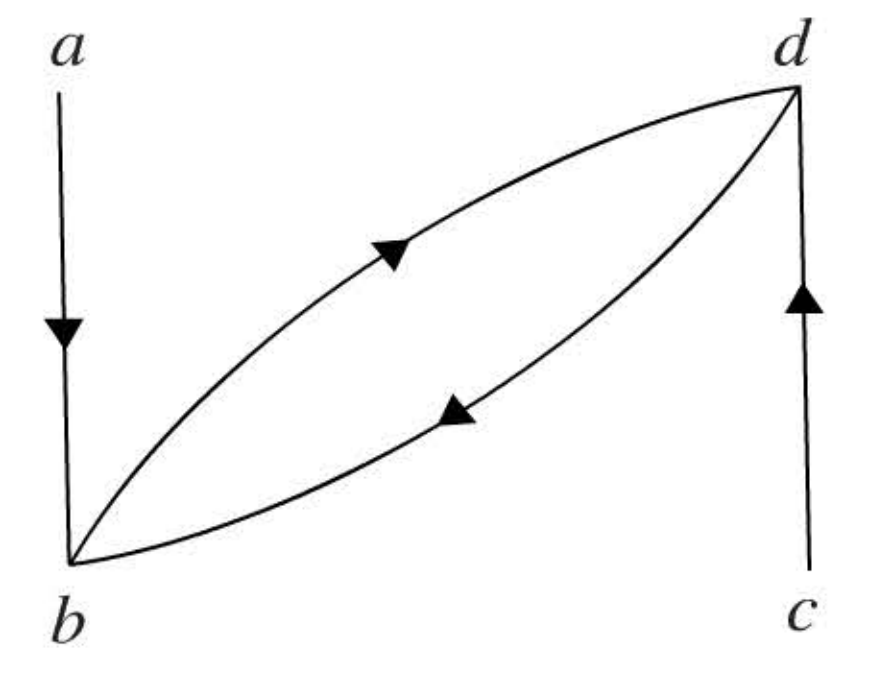
\includegraphics[width=5cm]{graphe.PNG}
\end{center}


On considère le dessin comme étant la représentation d'une relation binaire, que l'on note $\mathcal{R}$ . définie sur l'ensemble $S = \{ a;b;c;d\}$ .

\begin{enumerate}[\bfseries a.]
	\item 	Écrire tous les éléments qui sont en relation sou s la forme $x\mathcal{R}y$, avec $(x;y) \in S^2$ .
	\item 	La relation R est elle réflexive ?	
	\item 	La relation R est elle symétrique ?
	\item 	La relation R est elle transitive ?
	\item 	Au minimum, quelles flèches doit-on ajouter pour obtenir la représentation d'une
	relation réflexive ?
	\item Même question avec une relation symétrique. \\
\end{enumerate}
\exo{}

On considère l'\textit{arbre binaire suivant} et sur l'ensemble des nombres présents dans l'arbre, on définit une relation binaire : $x\mathcal{R}y$ si et seulement si $x=y$ on bien on peut passer de x à y ou de y à x par un chemin qui descend toujours par la droite.
\begin{center}
	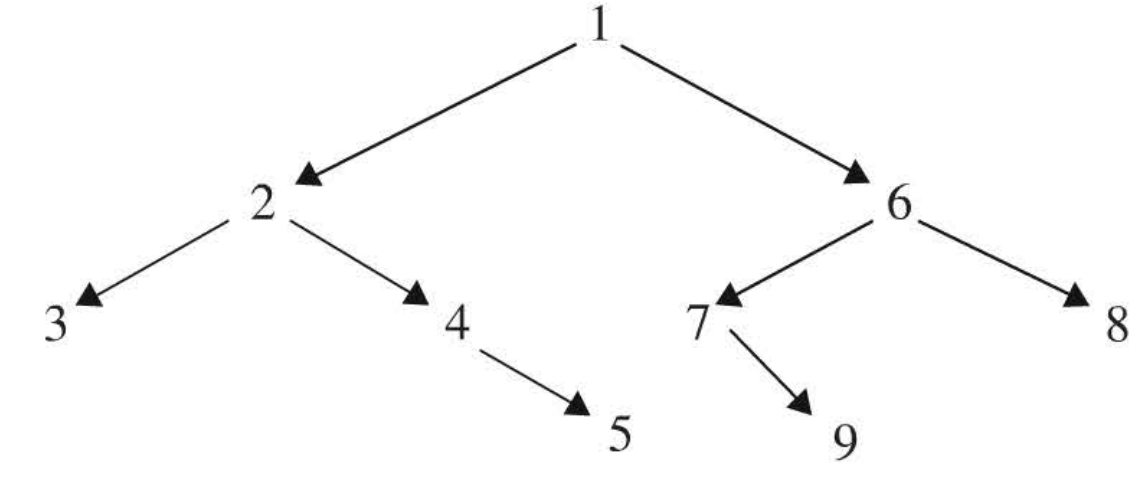
\includegraphics[width=8cm]{arbre.PNG}
\end{center}
\begin{enumerate}[\bfseries 1.]
	\item 	Expliquer pourquoi simplement à partir de sa définition on peut affirmer que $\mathcal{R}$ est réflexive et symétrique.
	\item 	Montrer que $\mathcal{R}$ est une relation d'équivalence.
	\item 	Regrouper sur le schéma ci-dessus les nombres équivalents.
\end{enumerate}
\end{document}
